%%%%%%%%%%%%%%%%%%%%%%%%%
% Set up to be stand alone document
% All declerations in the header to be removed when added into thesis
%%%%%%%%%%%%%%%%%%%%%%%%%
\documentclass[12pt]{article}

\usepackage{booktabs} % booktabs provides professional formatting commands for tables
\usepackage{amsmath} % amsmath provides extra maths symbols
\usepackage{textcomp} % textcomp provides extra text symbols (like a degrees celsius symbol)
\usepackage{../customisations}
\usepackage{natbib}

\title{$J$-band Sythentic Spectral Fitting}
\date{\today}

\begin{document}
\maketitle
%%%%%%%%%%%%%%%%%%%%%%%%%
% To be included when added into thesis
% \chapter{J-band Sythentic Spectral Fitting}

In this chapter I describe in detail the process by which I implement an analysis
routine to fit RSG sythetic spectra to observed data.
The spectra cover the $J$-band, spectifically the $1.16-1.22\mu$m region, where there are various prominent spectral features.
These spectral features, arising from elemental absorption, are compared in the observed and model spectra,
where the $\chi^{2}$-statistic is calcualted to asses the goodness of fit for each model.
The stellar parameters which are fit for in this analysis are global metallicitiy [Z], effective temperature (T$_{eff}$), microturblence ($\xi$) and surfance gravity ($log g$).
% In addition to these parameters, in the future I also hope to further develop this implementation to include the $\alpha$-to-iron ratio as a free parameter.
The observed spectra are fit with model spectra from a set of MARCS model atmospheres
\cite{2008A&A...486..951G}.

The wavelength range, over which to perform this analysis,
is chosen based on the spectral appearance of the region.
Typically, in the spectra of cool stars, dense molecular absorption fetuares dominate the spectrum which require high-resolution spectroscopy to distinguish individual features and derive stellar parameters~\cite{Cunha07, Davies09a, Davies09b}.
However, in this small wavelength range, the absorption is dominated by well separaeted elemental absorption features from iron, magnesium, silicon and titanium.
Therefore, the spectral resolution required in order to derive stellar paramters is significantly reduced.
This means that this analyis can be preformed with a relatively small amount of telescope time using multi-object spectrographs like the $K$-band multi-object spectrograph (KMOS)
or the multi-object spectrometer for infra-red exploration (MOSFIRE) and is therefore feasible for studies of red supergiant stars (RSGs) in external galaxies.

In addition to this, given the cool temperature of the outer layers of RSGs,
the peak brightness of a typical RSG is $\sim1.1\mu$m.
Combining this with the fact that dust attenuation is significanlty lower in the near-IR, compared to the optical regime, RSGs are ideal candidates to be studied at large distances.

Previous implemenations of this analysis include that of
\cite{2010MNRAS.407.1203D} and Gazak (2014).
This implemenation includes aspects of both of these previous implementations and could be described as a hybrid of the two.
I approach the implementation in a Bayesian manner which relies on good prior assumptions.
Eventually this analysis routine will be made publicly available which should encourage the community to engage with these routines.

In the remainder of this chapter I first describe the model grids and how they are used in~\ref{sub:model_grid}.
I then describe the contiuum fitting procedure in~\ref{sub:continuum_fitting},
and go on to detail the method for estimating the bestfit parameters in
~\ref{sub:best_fit_parameters}.
The testing process which these procedures have underwent is described in~\ref{sub:testing}, which also includes a comparison between the results produced using this implementation and those of the two previous implementations of the same analysis.
Finally, I conclude the chapter in~\ref{sub:conclusions}.

% Based on the work done by \cite{2010MNRAS.407.1203D} and Gazak (2014), I developed an implementation of the J-band synthetic spectral fitting software.
% This involves fitting the continuum between the observations and models and defining best fit model parameters for the stellar parameters,
% metallicity, effective temperature, surface gravity and microturbulence.
% The observations are fit with model spectra from a set of MARCS model atmospheres
% \cite{2008A&A...486..951G}.
% Spectra are extracted using the SUI code
% ~\cite{2012ApJ...751..156B,2013ApJ...764..115B,2014arXiv1412.6527B}
% with non-LTE corrections computed for iron, silicon and titanium.

\subsection{Model Grid} % (fold)
\label{sub:model_grid}
The model grids used in this analysis are based on model atmospheres computed from the
MARCS model atmospheres project~\citep{2008A&A...486..951G}.
These model atmospheres are one-dimensional models (i.e. spherically symmetric)
computed within local thermodynamic equiliburum (LTE).
% where standard mixing-length theory is assumed.
The MARCS models are particularly general and widely applicable to many different types of stars,
however, for the atmospheres of RSGs these assumptions are known to break down
~\citep{2002AN....323..213F,2010ASPC..425..124P}.
Therefore, in order to accurately analyse the spectra of RSGs additional corrections must be made.

The models used for this analysis are computed with a mass of $15M_{\odot}$.
The typical mass range of a RSG is within $8 \textendash40M_{\odot}$ however,
using this mass is applicable owing to the fact that altering the mass of these models affects only the extension
(or geometrical thickness) of the models which does not change for red giants or supergiants
~\citep{2010MNRAS.407.1203D}.

To improve the accuracy of the model atmospheres
non-LTE calculations have been performed for all elements which give rise to the diagnostic features within the wavelength range studied.
The corrections are applied to iron, titanium, silicon and magnesium
~\citep{2012ApJ...751..156B,2013ApJ...764..115B,2014arXiv1412.6527B}.
% and therefore all of the lines used as diagnostic lines have non-LTE calculations preformed.
Line profiles and non-LTE corrections are calculated using an updated version of the SIU code
~\citep{1999PhDT.........3R,2012ApJ...751..156B}.

The parameters of the resulting grid of model spectra are detailed in
Table~\ref{tb:grid}.
The model spectra are at $R~=~10\,000$,
which is chosen to be significantly higher than the typical resolution of the observed spectra
(i.e. $R\sim 3000$).
The sensitivity of each diagnositic line for a given free parameter is displayed in figures~\ref{fig:mod-z} through~\ref{fig:mod-micro}.

From an analysis of figures~\ref{fig:mod-z} and~\ref{fig:mod-g} it can be seen that the effect of increasing the metallicitiy of the models is similar to that of decreasing the surface gravity.
It is therefore expected that a degeneracy exists bewtween metallicitiy and surface gravity.
This degeneracy is explored further in~\ref{sub:testing}.
The effect of varying the temperature of the models changes the relative strengths of the lines of
different spectral species (e.g. iron to titanium).
This is clearly distinguishable from all the effects of all other parameters.
Increasing the microturblence has the effect of increasing the equivalent widths
of the strongest lines preferentially.
Therefore, features arising from the same element will be most sensitive to this
parameter.
This is illustrated by a comparison between the two strong iron lines in the left and
right panel of Figure~\ref{fig:mod-micro}.


\begin{table}
\caption{Model grid parameter space\label{tb:grid}}
 \note{This is the grid which I currently have.
       What does the most modern grid we have look like?}
\scriptsize
\begin{center}
\begin{tabular}{lccc}
 \hline
 \hline
Parameter & Abbreviation & Range & Increment \\
 \hline
Global Metallicitiy & $[Z]$ & $+1.0~\textendash~-1.0$ & 0.1\,$dex$ \\
Effective Temperature & $T_{eff}$ & $3400 ~ \textendash~4400$ & 100\,$K$ \\
Log gravity & $log g$ & $+1.0~ \textendash~-1.0$ & 0.25\,$dex$ \\
Microturblence & $\xi$ & $1.0~ \textendash~5.0$ & 0.2\,$km\,s^{-1}$ \\
 \hline
\end{tabular}
\end{center}
\end{table}


\begin{figure}
 \centering
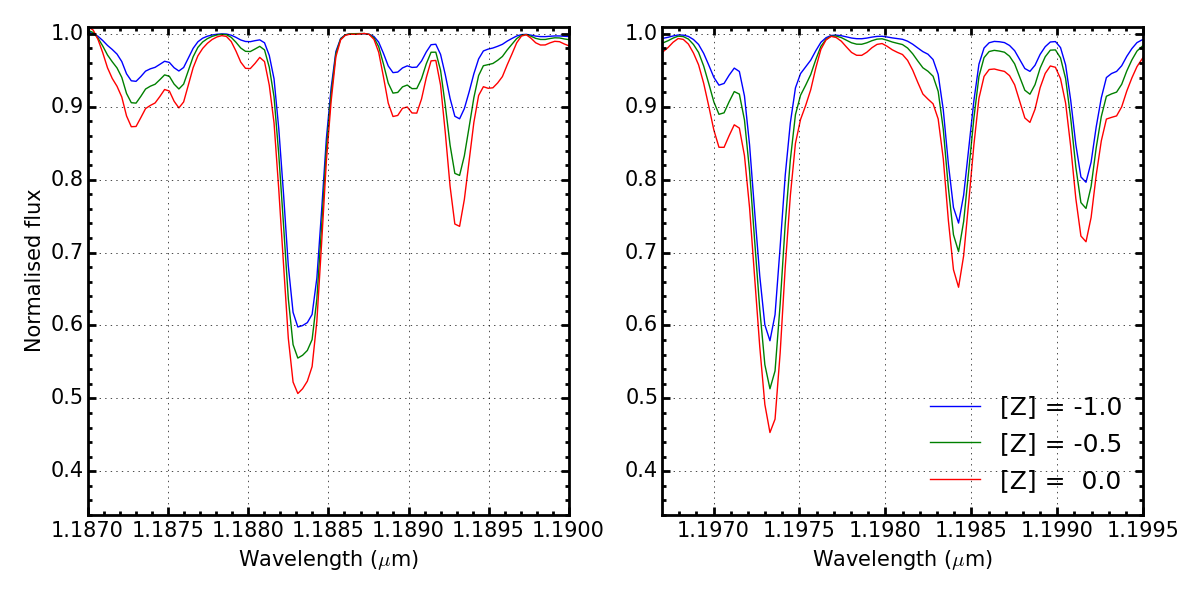
\includegraphics[width=\textwidth]{varyZv2}
\caption{
Three models where only the metallicitiy is varied.
Five diagnostic lines are shown in two panels.
Left: Fe\,I $\lambda$1.188285 and Ti\,I $\lambda$ 1.189289.
Right: Fe\,I $\lambda$ and Si\,I $\lambda\lambda$ 1.198419, 1.199157.\label{fig:mod-z}
         }
\end{figure}

\begin{figure}
 \centering
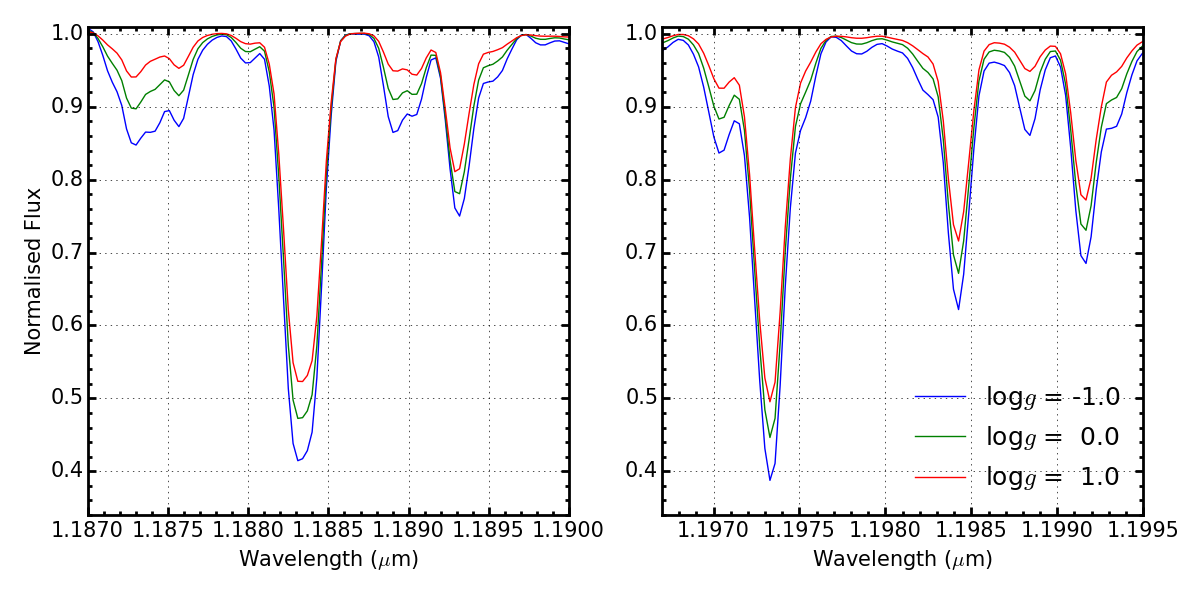
\includegraphics[width=\textwidth]{varygv2}
\caption{
As in Figure~\ref{fig:mod-z} where however surface gravity is varied.\label{fig:mod-g}
         }
\end{figure}

\begin{figure}
 \centering
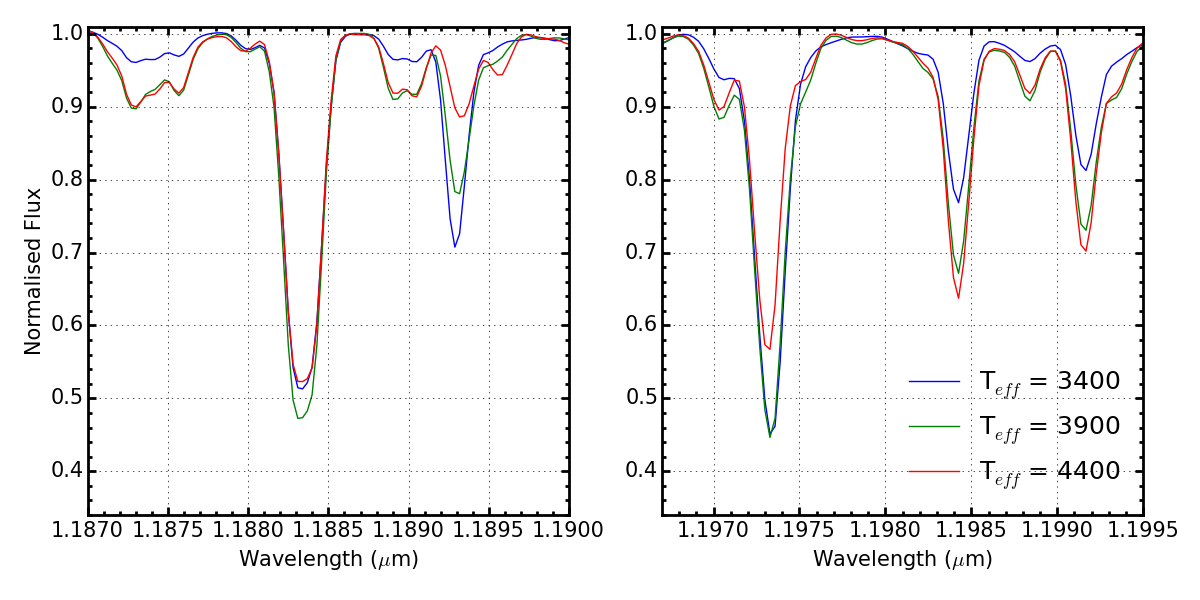
\includegraphics[width=\textwidth]{varyTv2}
\caption{
As in Figure~\ref{fig:mod-z} where however effective temperature is varied.\label{fig:mod-t}
         }
\end{figure}

\begin{figure}
 \centering
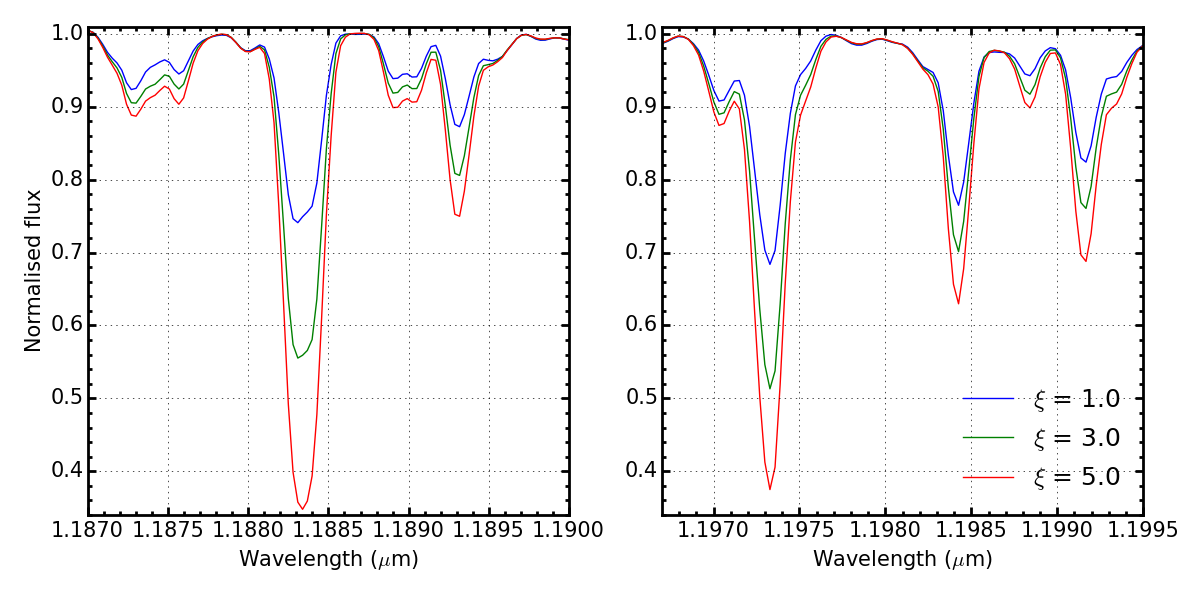
\includegraphics[width=\textwidth]{varymicrov2}
\caption{
As in Figure~\ref{fig:mod-z} where however microturblence is varied.\label{fig:mod-micro}
         }
\end{figure}

The current model grid is sufficent to explore the parameters for a typical RSG.
However, when using this technique at larger distances,
many different metallicity environments are encounted (e.g. I\,Zw\,18 with $Z=(1/32)Z_{\odot}$~\citep{1998ApJ...508..248V}).
In order to study these extemely low-metallicity systems,
the metallicity parameter space would need to be extended.
The $\alpha$-to-iron ratio of these stars is taken to be that of the solar value and is not left as a free parameter in the models.
This is applicable as young stars are known to have solar-like $\alpha$-to-iron ratios in different metallicitiy galaxies
~\citep[see tables 3 and 4 in][and references therin]{2015ApJ...806...21D}.

% \begin{itemize}
%     \item How are the grids generated?
%     \item What are the non-LTE corrections?
%     \item What do the current grids look like?
%     \item How could they be improved?
% \end{itemize}
% subsection model_grid (end)
\subsection{Continuum Fitting} % (fold)
\label{sub:continuum_fitting}

Accurately matching the continuum levels in the models with that of the observed
spectrum provides a base with which to anchor the diagnostic lines.
An incorrecly placed continuum level would bias the analysis and result in the
strength of the diagnostic lines being over or under estimated producing inaccurate stellar parameters.

% The continuum fitting procedure is important because determining the base of the
% diagnostic lines defines their overall strength which is used to distinguish
% between models.
There are many factors that effect the level of the continuum and continuum placement,
including the resolution of the observations as well as the stellar parameters themselves.
Therefore it is vital that when attempting to derive stellar paramters,
in crowded regions such as this, the continuum placement is performed
consistently and accurately.
Intrinsically, when stufying RSGs at medium resolution - owing  to their cool atmospheres -
there are many instances of blended spectral features.
At this resolution the density of blended spectral features creates a pseudo-continuum which, in practice,
is never at the ture continnum level.
Figure~\ref{fig:mod-res} illustrates the varying continuum levels for models where the resolution is varied and
Figure~\ref{fig:mod-zcont} shows this affect when varying only the metallicity.

\begin{figure}
 \centering
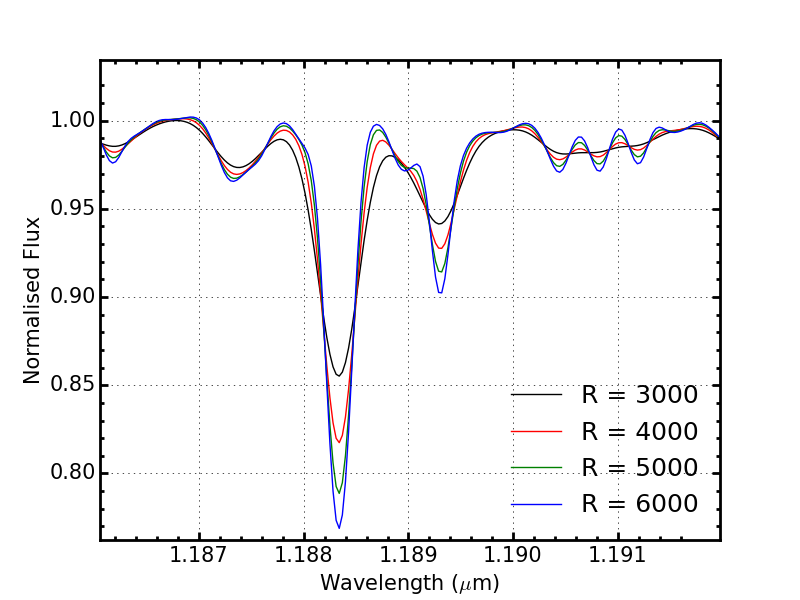
\includegraphics[width=\textwidth]{Resolution}
\caption{
One model degraded to four different resolution values.
This figure demonstrates the how the continuum level changes depending upon
the resolution of the spectrum.
We see at around 1.191$\mu$m at $R=3000$ the continuum level is perturbed by blended lines.\label{fig:mod-res}
         }
\end{figure}

\begin{figure}
 \centering
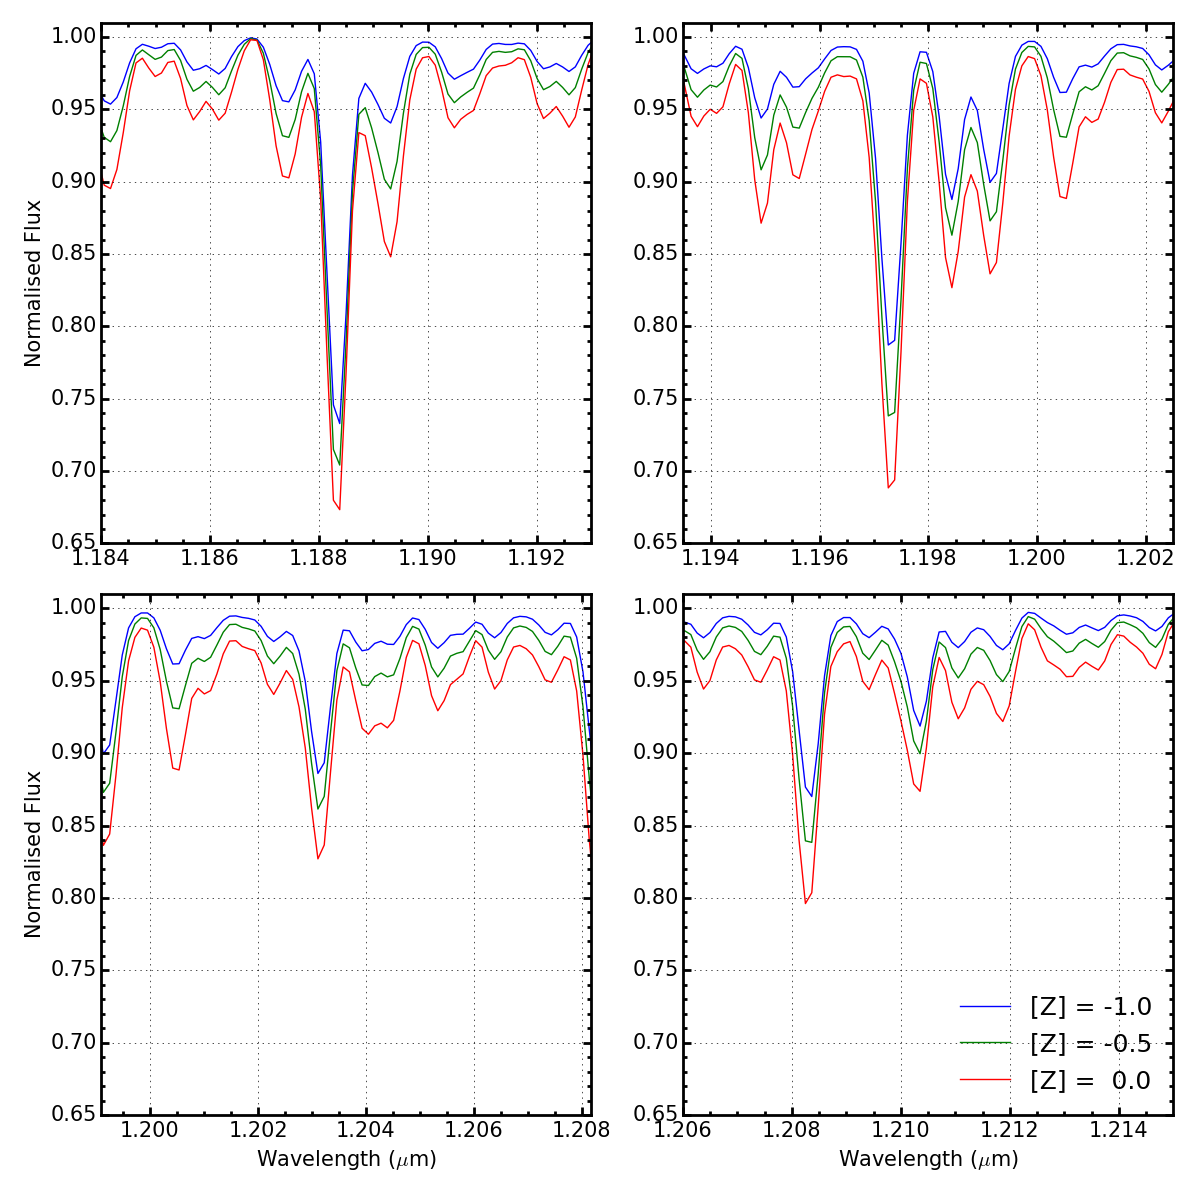
\includegraphics[width=\textwidth]{varyZ}
\caption{
Three models where only the metallicitiy is varied.
Each panel shows one or more diagnostic line.
Metallicity of the model intrinsically affects the continuum level of the spectrum,
such that at higher metallicities, there is greater departure from the true continuum level, which in the case of the models is 1.00.\label{fig:mod-zcont}
         }
\end{figure}


Given that it is impossible to know the true continuum level from any given observation,
the scaling applied must be consistent between the models and observations.
Scaling is required not only to match the levels of the continnum placement, but also to match the line strenghts between the models and observations.
Providing the treatment of the models and observations are consistent, the fact that the true continuum is never attained is not significant
\citep{2014ApJ...788...58G}.
For this procedure to work effectively,
the observed and model spectra should be at the same resolution,
have a consistent wavelength calibration
and have identical spectral sampling.

In order to account for differences in the spectral sampling of the observed and model spectra,
each model spectrum is resampled onto the wavelength scale of the observations by means of a spline interpolation routine.
The model spectrum is then degraded to the resolution of the observations by a
convolution with a Gaussian filter where the width of the Gaussian is defined by the observed resolution.
The resolution of the KMOS observations is estimated using the KMOS/esorex pipeline from arc lamp exposures at the appropriate rotator angle for the observations.
This is measured for each spectrograph and is assumed to be constant (to within $\pm 100$) across individual IFU's as well as across the detector.

% This is accounted for by degrading the sampling of the models to that of the observations by means of a linear interpolation.
% The sampling of the models are degraded to that of the observations by means of a cublic-spline interpolation.
To ensure the spectra are on the same wavelength scale, the observed specturm is cross-correlated with the model spectrum;
a shift is then applied to the observed spectrum in order to minimise the cross-correlation matrix.
This procedure is repeated until the shift between the observed and model spectra is less than $0.1\,pix$.
Over this small wavelength range, one would not expect significant variations in the spectral resolution of the observations to pertrub the cross-correlation.

Once the spectra have been correctly matched they are now suitable to be compared over the wavelength range $1.165-1.215\mu$m.
To estimate the amount of scaling required first I define the continuum width ($cw$) as:

\begin{equation}
    cw~=~\frac{\lambda}{R}, %\times S,
\end{equation}
\noindent where $R$ is the resolution of the spectrum and
$\lambda$ is the wavelength at which the width is taken
(in principle this wavelength varies across the spectrum, however, given our spectral window is sufficently small, I assume $\lambda~=~1.20\mu$m).
% and $S$ is a scale factor which takes the range $0.5 < S < 1.0$.
The continuum width is essentially the resolution element of the spectrum at a wavelength of
$\lambda~=~1.20\mu$m and defines the width in which we expect to find a combination of pixels from a spectral feature and a continuum point.

% multiplied by the scale factor $S$.
% In Gazak et al. (2015) this scale factor is fixed at 0.5.
% The scale factor is introduced because ... ?

The model spectrum is divided into wavelength slices each of width $cw\mu$m and the maximum of each slice is taken.
Using this array of maxima any major feature is systematically removed by rejecting data points more than 3$\sigma$ from the mean of the distribution.
Figure~\ref{fig:cw} illustrates the width of these slices and how this technique  removes prominent spectral features.
In this figure blue points represent the boundaries between the slices of witdh $cw\mu$m and the maximum of each slice is shown in red.
 % using this technique systematically removes absorption features from the spectrum.
% Any remaining features in this maximum spectrum are removed by rejecting outliers which are more than 3$\sigma$ from the mean of the distribution.
% In figure~\ref{fig:cw} the $cw~max.$ points have been through this procedure.
% This can be seen by noting that the cores of the absorption lines no $cw max.$
% points present.

\begin{figure}
 \centering
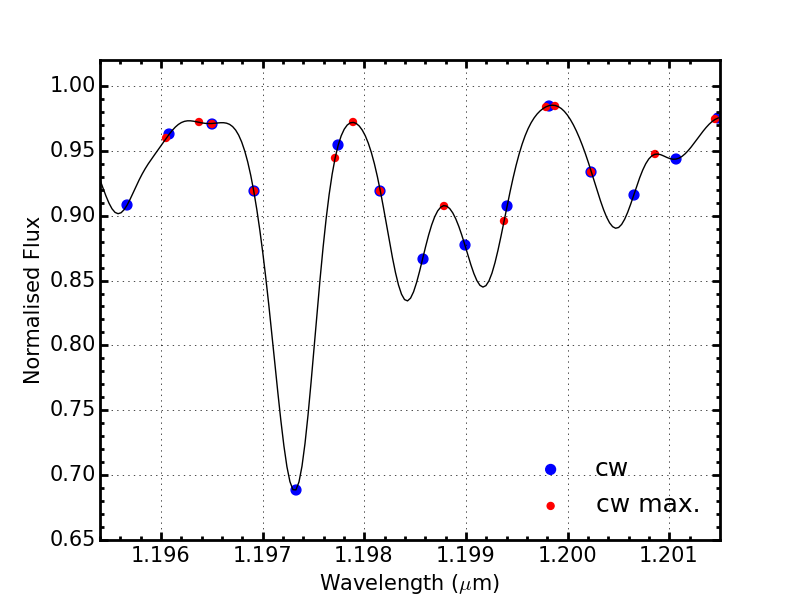
\includegraphics[width=\textwidth]{cw}
\caption[Illustration of continuum width slices and maxima]{
Illustration of the continuum width ($cw$) and slicing the model spectrum into regions of $cw\mu$m is able to remove structure in order to fit the continuum.
The solid black line shows an example of a model spectrum degraded to a resolution of 3000,
blue points show the boundaries between the slices and red points show the maximum of each slice.\label{fig:cw}
         }
\end{figure}


The remaining data points ($P_{cont}$) are used to derive an initial correction function
($cf_{1}$) by fitting a third-order polynomial to the ratio of the model to observed continuum points, defined using the equation:
\begin{equation}
    cf_{1}~=~f(\frac{F_{mod}(P_{cont})}{F_{obs}(P_{cont})})
\end{equation}

\noindent where $F_{mod}$ and $F_{obs}$ are the flux in the model and observed spectrum respectively.
The final correction function ($cf_{2}$), a refinement of $cf_{1}$,
is defined by removing any remaining outliers more than 3$\sigma$ from the mean of the correction function $cf_{1}$.
This method assumes that over the small wavelength range considered,
$cf_{1}$ does not vary significantly from the mean and as such, any significant deviation is considered originating from a spectral feature or noise.

The final correction function, $cf_{2}$,
is used to define the amount of scaling required for the model.
Figure~\ref{fig:cftaction} shows how the continuum fitting process works using a model spectrum as the observed spectrum (black) and a second model spectrum
(blue dashed) which is scaled to match the continuum level of the observed
(red dot-dashed).
It can be seen that the continuum placement of the example observed spectrum and that of the scaled model spectrum is well matched, even though the line strengths don't match well.

\begin{figure}
 \centering
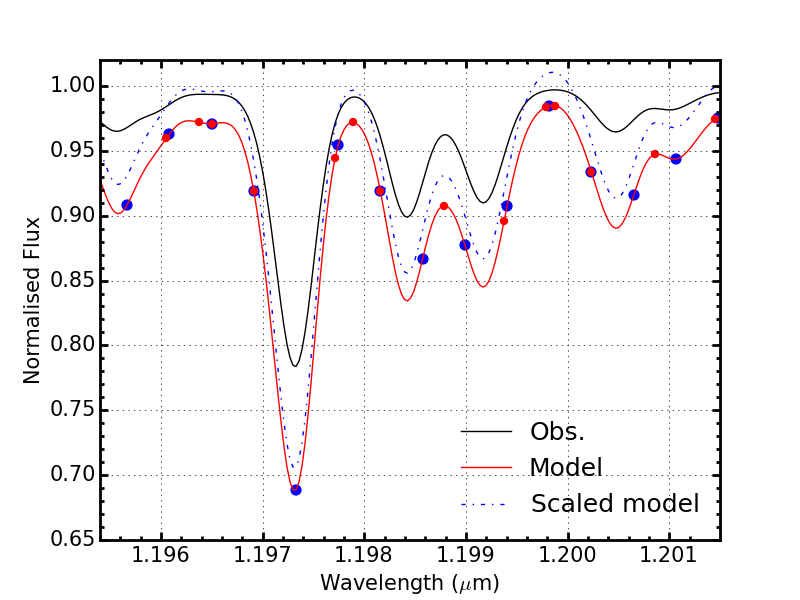
\includegraphics[width=\textwidth]{cftaction}
\caption[Example of continuum fitting]{
An example of how the continuum fitting procedure works using a model spectrum as
an example observed spectrum (black solid line)
and a separate model spectrum to match the level of the continuum.
The dashed blue spectrum denotes the model spectrum before any scaling has taken place.
The dot-dashed red spectrum denotes the model spectrum after the continuum fitting scaling has been applied.
The red and blue points the edges of the slices made and maxima of these regions respectively.\label{fig:cftaction}
         }
\end{figure}


% The green dashed line shows a third order polynomial fit to the ratio of the model spectrum to a simulated observed spectrum at only the red points ($~=~\frac{F_{mod}(cf_{1})}{F_{obs}(cf_{1})}$).

Alternative methods of continuum fitting are discussed in~\cite{2010MNRAS.407.1203D} and~\cite{2011A&A...527A..50E}.
These methods select pseduo-continuum pixels in the models based on ranking the model pixels and selecting a percentage of the pixels with the largest flux.
Providing the pixels from the model are selected in this manner and not those in the observations, this is a reliable method with which to derive the continuum level as demonstrated by~\cite{2015ApJ...806...21D}.
% \textbf{What advantage (if any) does the method applied here have over the one used in Davies et al. (2015 in prep.)?}

% subsection continuum_fitting (end)
\subsection{Best Fit Parameters} % (fold)
\label{sub:best_fit_parameters}

Best fit parameters are calculated using a chi-squared minimisation approach.
Each model is compared to the observed spectrum
and the chi-squared statistic is calculated using the equation,

\begin{equation}
    \chi^{2}~=~\frac{1}{N_{pix}}\sum\limits_{i}{\frac{(O_{i} - M_{i})^{2}}{\sigma^{2}}},
\end{equation}

where $N_{pix}$ is the number of pixels used and
$\sigma$ is determined by the S/N of the spectrum.
This statistic is calcualted over each of the diagnostic lines and here $N_{pix}$ is the total number of pixels used to perform this calculation.
Table~\ref{tb:lines} details the diagnostic lines used in this analysis.
The amount of continuum included to compute the $\chi^{2}$ is important to consider.
If this wavelength range is too small, the wings of the lines will be neglected,
which would discard vital information used to constrain the model parameters.
However, if too much of the psuedo-continuum is included, the parameters could be biased by noise features in the observations or by inaccuracies within the models.
For example,
~\cite{2014PhDT.........G} identify several spectral features present in the observed spectra which are missing in the model spectra.
The regions which are used in the $\chi^{2}$ calculation are hightlighed red in
figure~\ref{fig:lines}.
There are multiple cases where the diagnostic lines are sufficiently close together that, at R$\sim$3000,
the lines are not clearly separated.
In these instances, the most appropriate course of action is to define the region where the $\chi^{2}$ is computed over all of the lines in question and to deal with the region as a whole, as illustrated in Figure~\ref{fig:lines}.

\begin{figure}
 \centering
 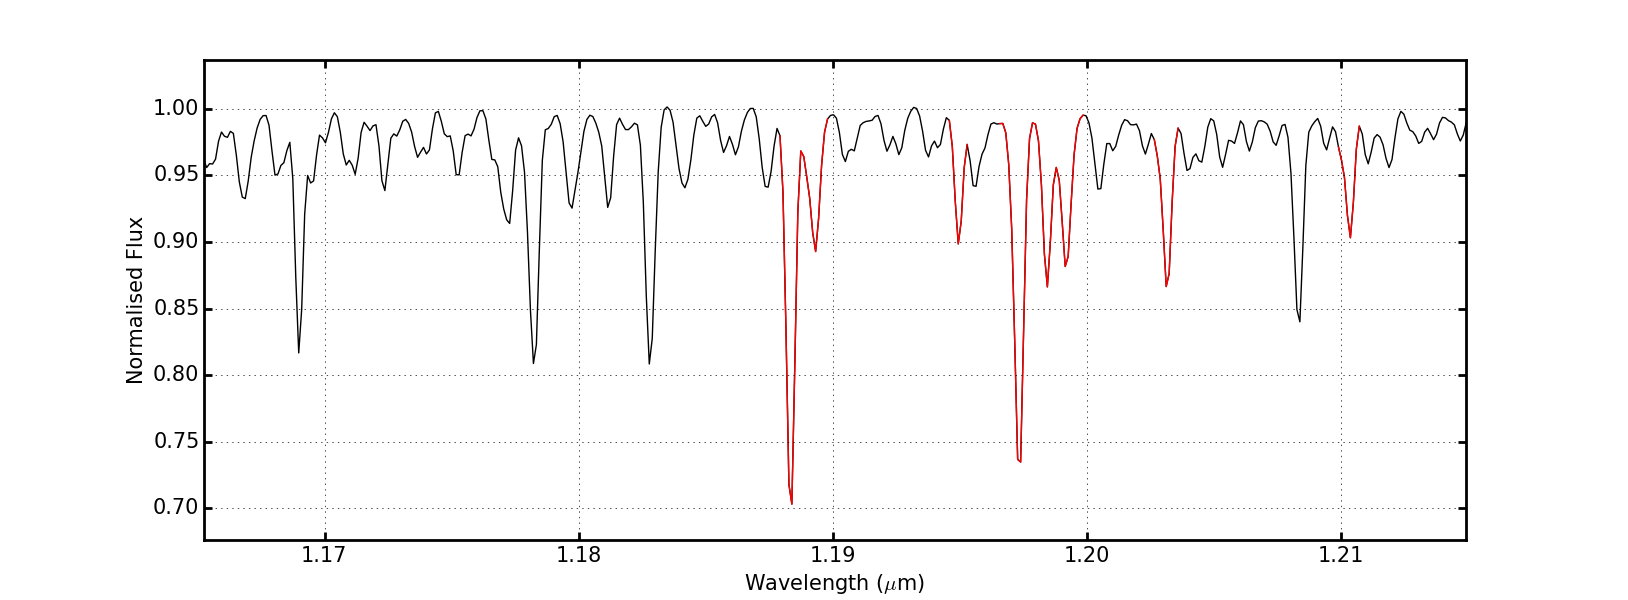
\includegraphics[width=\textwidth]{Diag-lines}
 \caption[Diagnostic lines]{
An example of a model spectrum, degraded and resampled to that of a typical observed spectrum (in this case NGC6822-RSG01), where the regions used to compute the $\chi^{2}$ calculation is highlighted in red.\label{fig:lines}
         }
\end{figure}

\begin{table}
\caption[Diagnostic lines]{Diagnostic lines\label{tb:lines}}
\scriptsize
\begin{center}
\begin{tabular}{cc}
 \hline
 \hline
Species & Line Centre \\
 \hline
Fe\,I & 1.188285 \\
Fe\,I & 1.197305 \\
Si\,I & 1.198419 \\
Si\,I & 1.199157 \\
Si\,I & 1.203151 \\
Si\,I & 1.210353 \\
Ti\,I & 1.189289 \\
Ti\,I & 1.194954 \\
Mg\,I & \\
Mg\,I & \\
 \hline
\end{tabular}
\end{center}
\end{table}

Each best fit parameter is estimated based on a weighted average,
where the weights are determined by the $\chi^{2}$ value of the model:

\begin{equation}
    w~=~exp(-\chi^{2}/2).
\end{equation}

The average is performed using the 100 models with the lowest $\chi^{2}$ value.

Errors on the parameters are determined by defining
$\Delta\chi^{2}~=~\chi^{2}_{min} + 3$.
The standard deviation of the models parameters for all models which have a
$\chi^{2}$ value within this range define the errors.
For a purely Gaussin distribution the 1$\sigma$ deviation is $\Delta\chi^{2}~=~2.3$.
However, assuming one of the diagnostic lines is only fit to within 2$\sigma$ while the rest being fit to within 1$\sigma$, we obtain $(n_{l}~-~1)~\times~1^{2}~+~1~\times~2^{2}~=~n_{l}~+~3$
where $n_{l}$ is the number of lines used.

As mentioned previouslly (in~\ref{sub:model_grid}) and as demonstrated in
~\cite{2015ApJ...806...21D} there exists a degeneracy between the effect of decreasing the metallicity and increasing the surface gravity of the models.
To help break this degeneracy, I implement an addition gravity restraint.
This works by calcualting the luminosity of the observed star using near-IR photometry and the bolometric correction given in~\cite{Davies13b}.
Having calculated the luminosity, the relationship,
\begin{equation}
    L~\propto~\frac{M\,T^{4}_{eff}}{g},
\end{equation}
can be used to restrict the $log\,g$-T$_{eff}$
parameter space using sensible limits for the mass of a RSG
($8~\leq~M/M_{\odot}~\leq~40$).
Where $M$ is the mass of the star,
$T_{eff}$ is the effective temperature and $g$ is the surface gravity of the star.
These regions of parameter space are rejected from the analysis as unphyiscal.


\subsection{Comparisons With Previous Implemetations} % (fold)
\label{sub:compare}
To increase confidence in the accuracy and reliability of this implemetation of the $J$-band synthetic spectral fitting routines,
where applicable, these routines have been compared to the results based on previous implemetations of this analysis.

To date, there are currently two other published implemtations using medium resolution $J$-band spectra of RSGs to derive stellar parameters,
that of~\cite{2010MNRAS.407.1203D} (DFK10) and that of~\cite{2014PhDT.........G}.
Both of these implemetations are subtly different and use different assumptions to derive the stellar parmaters.
They are both broadly based on the same techniques used in this analysis,
however, the main differences between the two methods are that DFK10 uses just the line strenghts of the diagnostic lines to calculate the $\chi^{2}$ statistic,
while G14 uses the entire $1.165-1.215\,\mu$m region (with some execptions).

In the current implementation, the diagnostic lines themselves are used to calculate the $\chi^{2}$ statistic.
This is prefered to the two afformentioned techniques for the following reasons:

1. The models used in the analsyis are not perfect reprsentations of RSG spectra.
The line list which builds these spectra are known to be incomplete and the effect of including these wavelength regions within the $\chi^{2}$ calculation could be to preturb the fit. G14 is very careful to exclude all known instances of missed lines within the models, however, this can not be assumed to be a complete consesus of missed lines.

2. Using the full line profile of the diagnostic lines provides information on the shape of the lines which using the line strength does not.

\subsubsection{DFK10} % (fold)
\label{sub:dfk10}
To date there have been several published articles using the DFK10 implemetation
~\citep{2010MNRAS.407.1203D,2015ApJ...803...14P,2015ApJ...806...21D}.
The original implemetation was updated and tested rigourously on VLT-XSHOOTER spectra of RSGs in the Magellanic clouds in
~\cite{2015ApJ...806...21D} and in~\cite{2015ApJ...803...14P} this was applied to KMOS spectra in NGC\,6822.
In this section we compare the analysis routine detailed above with that of DFK10 on the set of 10 RSG KMOS spectra in NGC\,6822.
Figure~\ref{fig:n6822DFK} shows the comparison of the output parmaters of the stars in this sample for the two analysis routines.
This figure shows that the agreement between the two routines is acceptable for all stellar parameters.
The mean of each of the parmeters is calculated in Table~\ref{tb:DFK10} and is shown to agree within the errors.

\begin{figure}
 \centering
 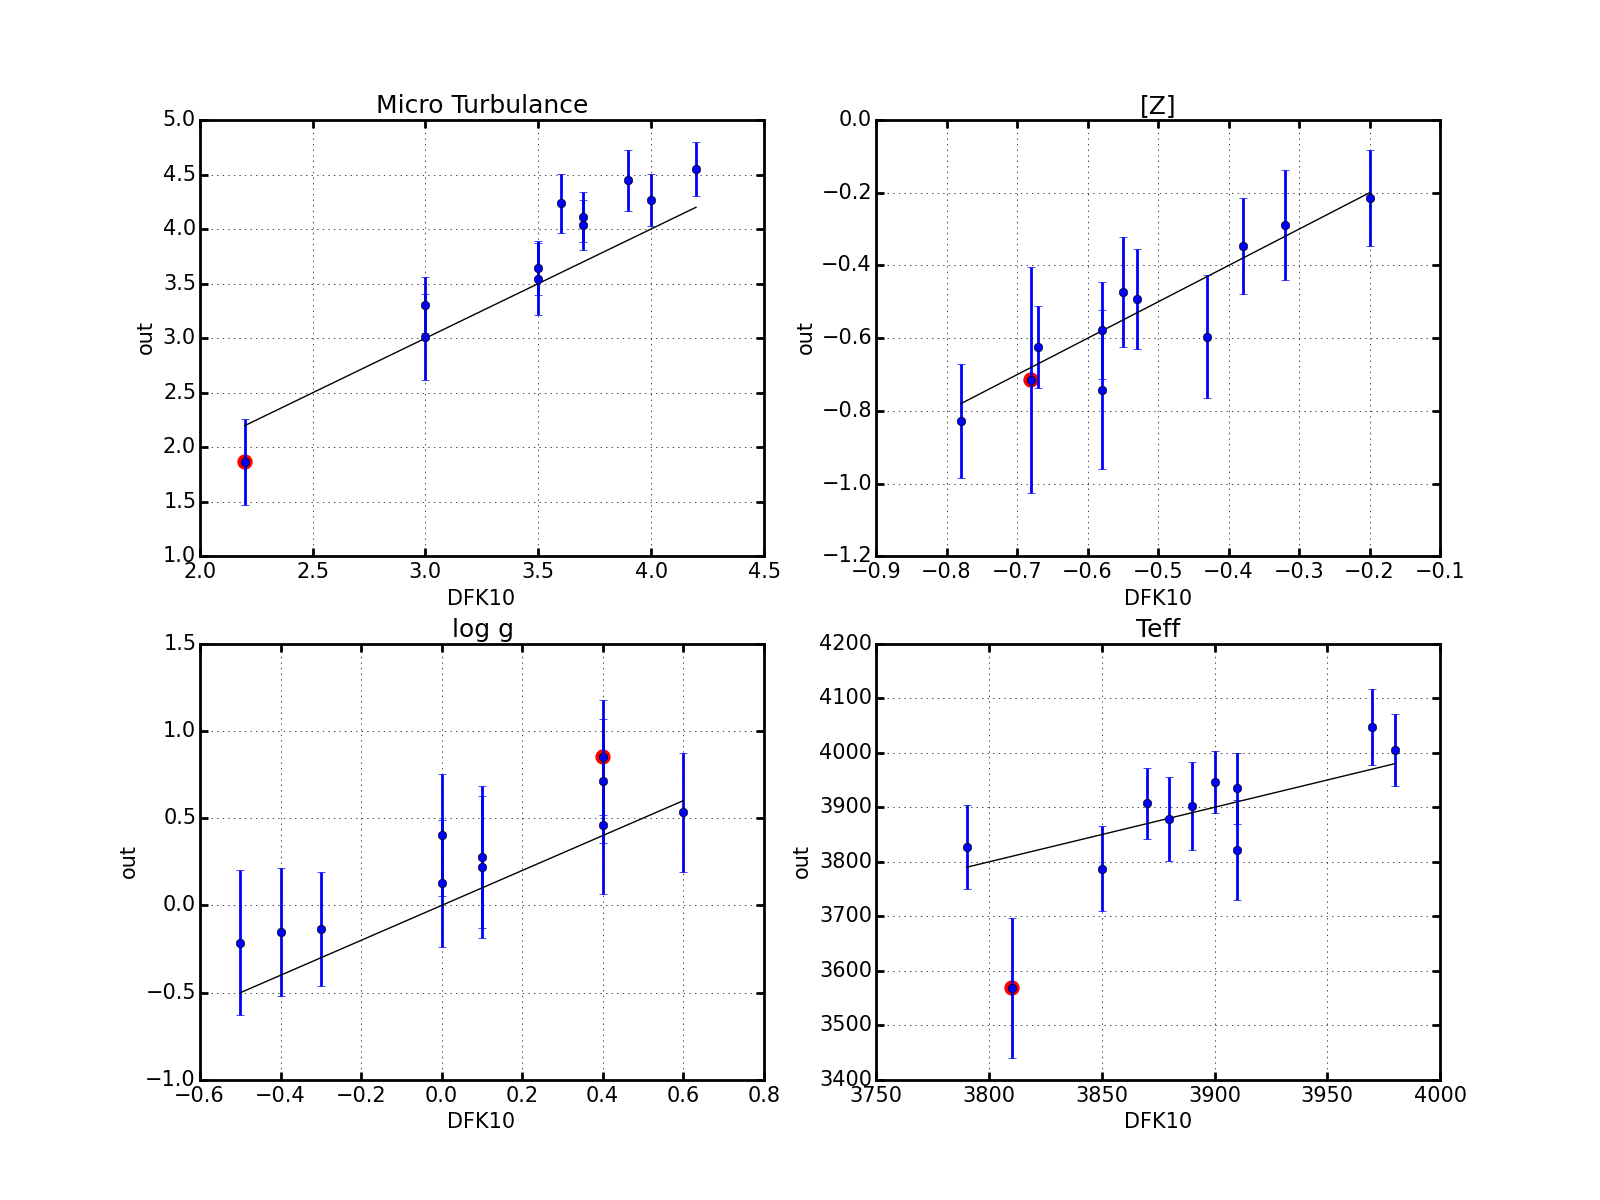
\includegraphics[width=\textwidth]{compare-DFK10}
 \caption[NGC\,6822 DFK10]{
A comparison between the parameters derived for 11 RSGs in NGC\,6822.
DFK10 results are those published in~\cite{2015ApJ...803...14P}.\label{fig:n6822DFK}
         }
\end{figure}

\begin{table}
\caption[Parameter comparisons DFK10]{Average parameters for 10 RSGs in NGC\,6822 using the DFK10 implementation and the implemetation discribed here\label{tb:DFK10}}
\scriptsize
\begin{center}
\begin{tabular}{ccc}
 \hline
 \hline
Parameter & DFK10 Average & Patrick Average \\
 \hline
[Z]       & $-0.52~\pm~0.16$ &  \\
T$_{eff}$ & $3887~\pm~55$ &  \\
$log\,g$  & $0.1~\pm~0.3$ &  \\
$\xi$     & $3.9~\pm~0.5$ &  \\
 \hline
\end{tabular}
\end{center}
\end{table}
% subsection dfk10 (end)

\subsection{G14} % (fold)
\label{sub:g14}
The second implementation of the $J$-band analysis technique using $J$-band spectra of RSGs was that presented and rigorously tested in~\cite{2014PhDT.........G}.
This implemetation was set up to be complemetary to that of DFK10 and was tested on high resolution spectra of RSGs in the Perseus OB-1 cluster.
In addition to this, this analysis was applied to KMOS spectra of 27 RSGs of NGC\,300
\citep{...}.

Stellar parameters have been for all spectra in NGC\,300 using the presented analysis.
In figure~\ref{fig:n300G14} I comapre the results derived using the analysis presented here with those published in~\citep{...}.
Table~\ref{tb:G14} shows a comparison between the the mean and standard deviation of the four paramaters.
The metallicity gradient is also derived for these observations and is found to compare ...

As part of the analyis G14 also fit for the resolution of the observations as a free parameter.
The resolution for each spectrum is compared to that of the values quoted in the KMOS arc-lamp calibrations.

\begin{figure}
 \centering
 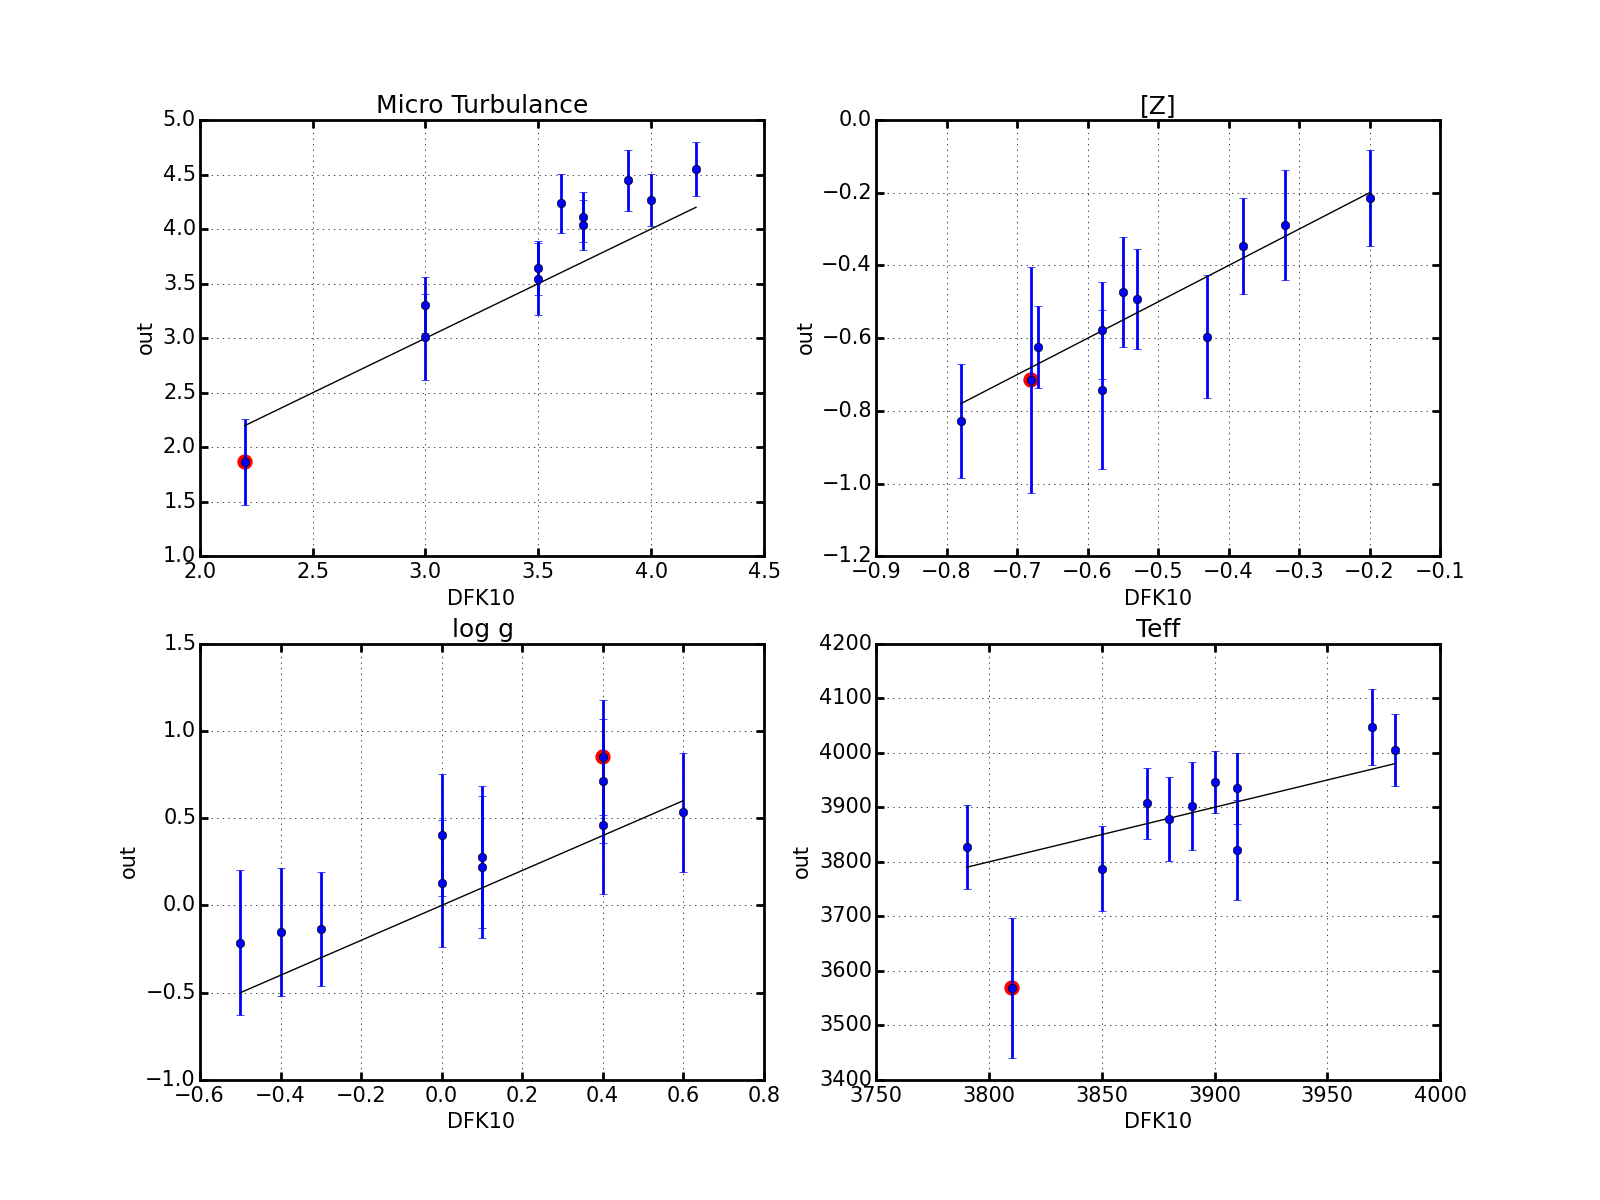
\includegraphics[width=\textwidth]{compare-DFK10}
 \caption[NGC\,300 G14]{
A comparison between the parameters derived for 27 RSGs in NGC\,300.
DFK10 results are those published in~\cite{...}.
\textbf{Placeholder!}\label{fig:n300G14}
         }
\end{figure}

\begin{table}
\caption[Parameter comparisons G14]{Average parameters for 27 RSGs in NGC\,300 using the G14 implementation and the implemetation discribed here
\textbf{Placeholder!}\label{tb:G14}}
\scriptsize
\begin{center}
\begin{tabular}{ccc}
 \hline
 \hline
Parameter & G14 Average & Patrick Average \\
 \hline
[Z]       & $-0.52~\pm~0.16$ &  \\
T$_{eff}$ & $3887~\pm~55$ &  \\
$log\,g$  & $0.1~\pm~0.3$ &  \\
$\xi$     & $3.9~\pm~0.5$ &  \\
 \hline
\end{tabular}
\end{center}
\end{table}
% subsection g14 (end)
% subsection compare (end)

\subsection{Conclusions} % (fold)
\label{sub:conclusions}

% subsection conclusions (end)
% subsection best_fit_parameters (end)
\bibliography{../journals}{}
\bibliographystyle{apalike}
%%%%%%%%%%%%%%%%%%%%%%%%%
% To be removed when added into thesis
\end{document}
%%%%%%%%%%%%%%%%%%%%%%%%%